\documentclass[11pt,a4paper]{article}
\usepackage[utf8]{inputenc}
\usepackage[T1]{fontenc}
\usepackage{amsfonts}
\usepackage{amssymb}
\usepackage{mdframed}
\usepackage{tikz}
\usepackage{tkz-tab}
\usepackage{wrapfig}
\usepackage{pgfplots}
\usepackage{xcolor}
\usepackage{fancyhdr}
\usepackage{lastpage}
\usepackage[fleqn]{amsmath}
\setlength{\mathindent}{0pt}

% Défini les couleurs pour les graphiques
\definecolor{dark_green}{HTML}{008000}

% Extensions
\RequirePackage{geometry} 
\geometry{tmargin=1cm,bmargin=1.9cm,lmargin=1.9cm,rmargin=1.9cm}

% Paramètres du titre
\def\classe{$1^{\text{re}}$ Spécialité mathématiques}
\def\titre{Nombre dérivé et applications}
\def\theme{Analyse - Cours et démonstrations}

% Paramètres de numérotation des pages
\fancypagestyle{custom}{
  \fancyhf{}
  \renewcommand{\headrulewidth}{0pt}
  \lfoot{Analyse - Cours et démos}
  \cfoot{Nombre dérivé et applications}
  \rfoot{\thepage/\pageref{LastPage}}
}

\usepackage{titlesec} % Pour personnaliser les titres
\usepackage{xcolor} % Pour définir des couleurs

\title{\titre}
\author{\classe \\ \theme}
\date{}

\renewcommand{\familydefault}{\sfdefault}

% Styles pour les mdframed
\mdfdefinestyle{definitionStyle}{
    leftline=true,
    rightline=false,
    topline=false,
    bottomline=false,
    linewidth=2pt,
    linecolor=black,
    innertopmargin=0pt,
    innerbottommargin=0pt,
    innerrightmargin=0pt,
    innerleftmargin=5pt,
}

\mdfdefinestyle{proprieteStyle}{
    linewidth=1pt,
    linecolor=black,
    innertopmargin=5pt,
    innerbottommargin=5pt,
    innerrightmargin=5pt,
    innerleftmargin=5pt,
}

% Supprime l'indentation des paragraphes
\setlength{\parindent}{0pt}

\begin{document}

\maketitle
\pagestyle{custom}
\thispagestyle{custom}

Pour la suite du cours, on a $f$ une fonction définie sur un intervalle $I$ et on note $C_f$ sa courbe représentative ainsi que $a$ un réel appartenant à $I$ et on note $A$ le point de $C_f$ d'abscisse $a$.

\section*{I. Taux de variation et nombre dérivé d'une fonction}
\subsection*{1. Taux de variation d'une fonction entre deux réels}

\begin{mdframed}[style=definitionStyle]
    \textbf{Définition :} ~\\
    Soit $f$ une fonction définie sur un intervalle $I$ et $a$ et $b$ sont deux réels de $I$. ~\\
    On appelle taux de variation ou taux d'accroissement de $f$ entre $a$ et $b$ le nombre $\displaystyle{\frac{f(b)-f(a)}{b-a}}$.
\end{mdframed}

\textbf{Interprétation géométrique :} Le taux de variation de $f$ entre $a$ et $b$ correspond au coefficient directeur
de la droite $(AB)$ avec $A(a; f(a))$ et $B(b; f(b))$. \\

\textbf{Interprétation cinématique :} Si la fonction $f$ représente la distance parcourue par un mobile en fonction du temps, le taux de variation de $f$ entre $a$ et $b$ représente la vitesse moyenne entre les instants $a$ et $b$.

\subsection*{2. Notion de nombre dérivé}

\begin{mdframed}[style=definitionStyle]
    \textbf{Définition :} ~\\
    On considère une fonction $f$ définie sur un intervalle $I$. \\
    Soit $a$ un réel de $I$ et $h$ un réel non nul tel que $a+h\in I$.

    On dit que la fonction $f$ est dérivable en $a$ lorsque le taux de variation de $f$ entre les réels $a$ et $a+h$ tend vers un nombre réel $L$ lorsque $h$ se rapproche de $0$.

    Dans ce cas, ce réel est appelé nombre dérivé de $f$ en $a$ et on le note $f'(a)$.

    On écrit alors $\displaystyle{\lim_{h\to0}%
            \frac{f(a+h)-f(a)}{h}}=f'(a)$.
\end{mdframed}

\textbf{Interprétation cinématique :} \\
Lorsque $f$ est une fonction représentant la distance parcourue par un mobile en fonction du temps :
\begin{itemize}
    \item le quotient $\frac{f(a+h)-f(a)}{h}$ représente la vitesse moyenne entre les instants $a$ et $a+h$.
    \item le nombre dérivé $\displaystyle\lim_{h\to0}$$\frac{f(a+h)-f(a)}{h}=f'(a)$ représente la vitesse instantanée à l'instant $t=a$.
\end{itemize}

\newpage

\section*{II. Tangente à une courbe en un point $\boldsymbol{A}$}

\begin{minipage}{0.55\textwidth}
    Sur la figure ci-contre : $\color{dark_green}A(a;f(a))$ et $\color{blue}H(a+h;f(a+h))$. \\

    Le coefficient directeur de la droite $(AH)$ est $\frac{y_H-y_A}{x_H-x_A}=\frac{f(a+h)-f(a)}{a+h-a}=\frac{f(a+h)-f(a)}{h}$. \\

    Que se passe-t-il lorsque $H$ se rapproche de plus en plus du point $A$, autrement dit lorsque $h$ se rapproche de plus en plus de $0$ ? \\

    Si $h$ tend vers $0$, la droite $(AM)$ se rapproche de la tangente à la courbe en $A$. Donc $\displaystyle{\lim_{h\to0}%
            \frac{f(a+h)-f(a)}{h}}$ noté $f'(a)$ correspond au coefficient directeur de la tangente. \\
\end{minipage}
\hspace{0.05\textwidth}
\begin{minipage}{0.4\textwidth}
    \begin{tikzpicture}
        \begin{axis}[
                axis lines=middle,
                xmin=-3, xmax=6,
                ymin=-3, ymax=8,
                xtick=\empty,
                ytick=\empty
            ]
            \draw[dashed, thin, dark_green] (axis cs:3,0) -- (axis cs:3,3);
            \draw[dashed, thin, dark_green] (axis cs:0,3) -- (axis cs:3,3);
            \draw[dashed, thin, blue] (axis cs:3.8,0) -- (axis cs:3.8,5.24);
            \draw[dashed, thin, blue] (axis cs:0,5.24) -- (axis cs:3.8,5.24);
            \addplot[smooth, thick, red, domain=-2:6] {(x-2)^2+2};
            \addplot[mark=x, mark size=3, only marks] coordinates {(3,3)};
            \addplot[mark=x, mark size=3, only marks] coordinates {(3.8,5.24)};
            \node[label={120:$\color{dark_green}A$}] at (axis cs:3.1,2.9) {};
            \node[label={-30:$\color{blue}H$}] at (axis cs:3.7,5.6) {};
            \node[label={-170:$\color{blue}f(a+h)$}] at (axis cs:0.2,5.8) {};
            \node[label={-170:$\color{dark_green}f(a)$}] at (axis cs:0.2,3.6) {};
            \node[label={-170:$\color{blue}a+h$}] at (axis cs:5,0.16) {};
            \node[label={-170:$\color{dark_green}a$}] at (axis cs:3.5,0) {};
            \node[label={90:$\color{red}C_f$}] at (axis cs:-0.8,6) {};
            \node[label={-120:$0$}] at (axis cs:0.1, 0.2) {};
        \end{axis}
    \end{tikzpicture}
\end{minipage} \\


\begin{mdframed}[style=definitionStyle]
    \textbf{Définition :} ~\\
    Lorsque $f$ est dérivable en $a$, on appelle tangente à la courbe $C_f$ au point d'abscisse $a$, la droite $T$ passant par $A(a;f(a))$ dont le coefficient directeur est $f'(a)$.
\end{mdframed}

\begin{minipage}{0.4\textwidth}
    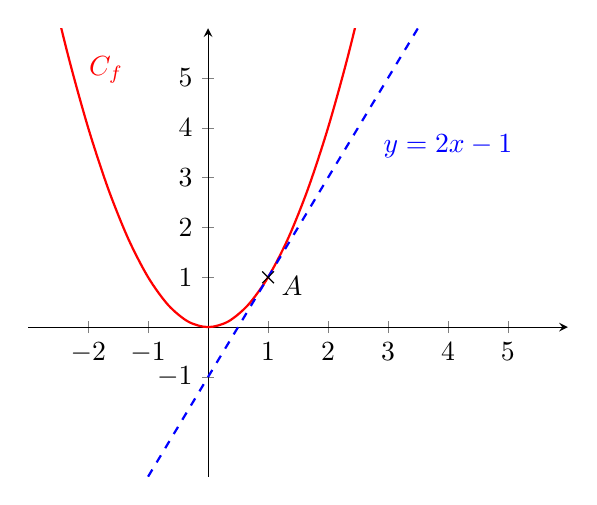
\begin{tikzpicture}
        \begin{axis}[
                axis lines=middle,
                xmin=-3, xmax=6,
                ymin=-3, ymax=6,
                xtick={-2, -1, 1, 2, 3, 4, 5},
                ytick={-1, 1, 2, 3, 4, 5}
            ]
            \addplot[smooth, thick, red, domain=-4:4] {x^2};
            \addplot[dashed, thick, blue, domain=-4:4] {2*x - 1};
            \addplot[mark=x, mark size=3, only marks] coordinates {(1,1)};
            \node[label={90:$\color{blue}y=2x-1$}] at (axis cs:4,3) {};
            \node[label={-90:$A$}] at (axis cs:1.4,1.4) {};
            \node[label={90:$\color{red}C_f$}] at (axis cs:-1.7,4.5) {};
        \end{axis}
    \end{tikzpicture}
\end{minipage}
\hspace{0.05\textwidth}
\begin{minipage}{0.55\textwidth}
    \textbf{Exemple :} Soit $f$ définie sur $\mathbb{R}$ par $f(x)=x^2$ et $C_f$ sa courbe représentative. \\

    L'équation de la tangente à la courbe $C_f$ au point $A$ d'abscisse $1$ est de la forme $y=mx+p$ avec $m=f'(1)=2$. \\

    L'équation devient $y=2x+p$. On peut remplacer $x$ par $1$ et $y$ par $f(1)=1^2=1$. ~\\

    Ainsi, $1=2\times1+p\Leftrightarrow1=2+p\Leftrightarrow p=-1$.
    L'équation de la tangente est $y=2x-1$.
\end{minipage}

\begin{mdframed}[style=proprieteStyle]
    \textbf{Propriété :} ~\\
    Soit $f$ une fonction dérivable en $a$, de courbe représentative $C_f$. \\
    L'équation de la tangente à $C_f$ au point $A$ d'abscisse $a$ est donné par la formule $y=f'(a)(x-a)+f(a)$.
\end{mdframed}

\underline{Démonstration :} \\

L'équation de la tangente à la courbe $C_f$ au point $A$ d'abscisse $a$ est de la forme $y=mx+p$ avec $m=f'(a)$. \\
L'équation devient $y=f'(a)x+p$. \\
On peut remplacer $x$ par $a$ et $y$ par $f(a)$.
\vspace{-8pt}
\begin{align*}
    \text{Ainsi,}            & f(a)=f'(a)a+p \\
    \Leftrightarrow \text{ } & f(a)-f'(a)a=p
\end{align*}
\vspace{-30pt}
\begin{align*}
    \text{L'équation de la tangente est donc } & y= f'(a)x+f(a)-f'(a)a \\
    \Leftrightarrow \text{ }                   & y =f'(a)(x-a)+f(a)
\end{align*}

\end{document}